\chapter{Conclusion and Future Work}

For implementing the RL algorithms to learn schedules, we need a discrete event simulator 
that drives the algorithm. First phase of the BTP, focuses on implementing the simulator and 
understanding the prior work in detail. The second phase is focused more on the implementation of the 
algorithm and experiments. 

\vspace{\baselineskip}
The algorithm discussed in the report treats each train as a single agent, So whole system i.e. 
whole network and trains, is a multiagent environment. First the algorithm discusses about the 
local state space of each train , actions and policy ($\epsilon$ - greedy policy) and the objective
function used in this study. Next we discuss about the Sarsa($\lambda$) algorithm with reward as the negative 
of the objective function. This algorithm does not perform well, since the reward is at the end of the episode, 
and back-propagation of reward through the trajectory is not possible. So we defined \textbf{proxy reward} which 
captures the probability of state-action pair to end up in a successful episode. Using the proxy reward,
we defined Q-values in two different ways. First one looks at success probability of current state-action pair 
and success probability of its neighbors. Second one looks all the way down to trajectory instead of 
two step reward functions. Second definition of Q-value, gives better results.

% \vspace{-5cm}
\vspace{\baselineskip}
The algorithms are tested on three Hypothetical datasets. Testing is done on standard railway system 
(without external delay) and 
also by introducing 20\% random delay in the running time of trains. From results, we can conclude that the 
proposed definition of Q-value performs better.One of the advantage of the study is \textbf{Transfer learning}
in which training is done on one 
problem instance and testing is done on similar problem instance.
% \vspace{15cm}

% \begin{figure}[h]
    % \centering
    % 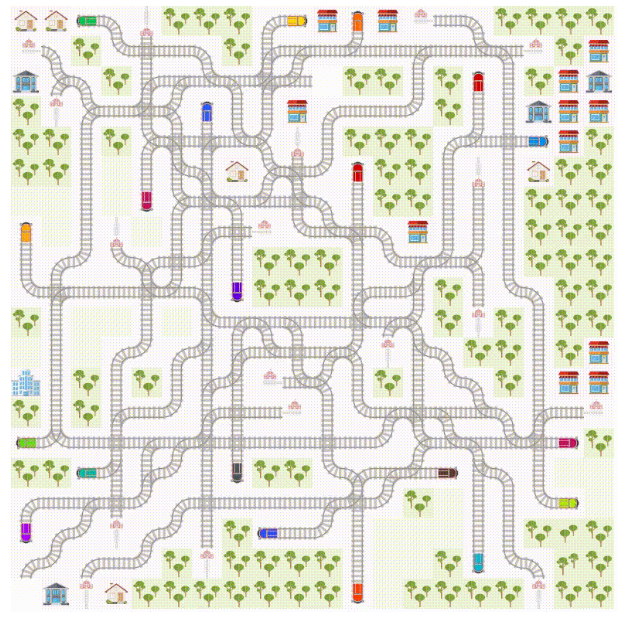
\includegraphics[width=0.5\textwidth]{flatland}
    % \caption{ Flatland environment, railway network as grid world\cite{ARTICLE:3} }
    % \label{flatland}
%   \end{figure}
\vspace{\baselineskip}
The algorithm in this report focuses on finding schedules for railway lines instead of railway network.
In the future, we can extend the algorithm to work for railway networks. 

\vspace{\baselineskip}
Recently, AICrowd developed a \textbf{flatland environment}\cite{ARTICLE:3} to foster progress in \textbf{multi-agent
reinforcement learning for any re-scheduling problem (RSP)}. They have defined
the railway network in a complete new setting using grid instead of graph. Future course of the project is to 
work on more general problem of flatland (which can be used for solve railway scheduling, 
transport management problems) and develop algorithms that can solve scheduling problem over 
grid world having multiple agents. 

